\section{Instrument Design}
\label{sec:instrument-design}

HunStat2 is a single-channel, three-electrode potentiostat built directly
from the Analog Devices AD5940/AD5941 datasheet~\cite{devices2024ad5940},
standard three-electrode potentiostat design practice, and the Analog
Devices AD5940 evaluation-kit reference firmware~\cite{ad5940_examples_github}.

\subsection{Instrument}
\label{sec:device-photo}
Figure~\ref{fig:device-photo} shows the assembled instrument used for every
measurement in this paper and in the two companion
manuscripts~\cite{clement2026linearity,clement2026architecture}: the AD5941
AFE and Seeed Studio XIAO RP2040 MCU on the \texttt{STEI\_Bstat\_v1.2}
carrier board, with the working/reference/counter (WE/RE/CE) electrode
header used to connect the dummy cell.

\begin{figure}[h]
\centering
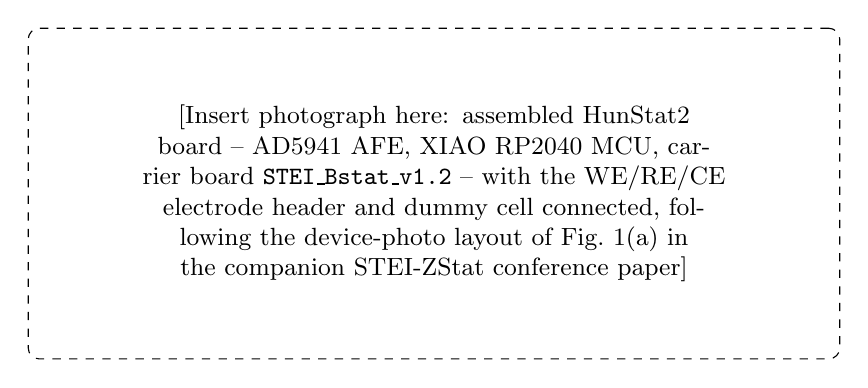
\begin{tikzpicture}
\node[draw, dashed, rounded corners, minimum width=0.85\linewidth,
  minimum height=4.2cm, align=center, font=\small, text width=0.7\linewidth]
  (photo) {[Insert photograph here: assembled HunStat2 board --
  AD5941 AFE, XIAO RP2040 MCU, carrier board \texttt{STEI\_Bstat\_v1.2} --
  with the WE/RE/CE electrode header and dummy cell connected, following
  the device-photo layout of Fig.~1(a) in the companion STEI-ZStat
  conference paper]};
\end{tikzpicture}
\caption{HunStat2, the AD5941/RP2040 potentiostat under test: assembled
board with the AD5941 AFE, XIAO RP2040 MCU, and WE/RE/CE electrode header
used to connect the dummy cell of Section~\ref{sec:protocol}.}
\label{fig:device-photo}
\end{figure}

\subsection{Components}
\label{sec:components}
Table~\ref{tab:components} lists the instrument's principal components.
The AD5941 supplies the entire analog measurement chain -- both excitation
loops, both transimpedance stages, the ADC, and the DFT engine -- as
characterized, off-the-shelf silicon~\cite{devices2024ad5940}; the RP2040
MCU is responsible only for register sequencing, host communication, and
unit conversion. This is exactly why the defects diagnosed in this paper
are firmware defects, not analog ones: both are a matter of which of the
AD5941's own, correctly-functioning internal paths the firmware asks for,
and how it interprets the code that path returns.

\begin{table}[h]
\centering
\footnotesize
\setlength{\tabcolsep}{4pt}
\caption{Principal components of the HunStat2 instrument.}
\label{tab:components}
\begin{threeparttable}
\begin{tabular}{@{}p{0.24\linewidth}p{0.68\linewidth}@{}}
\toprule
Component & Role / key specification \\
\midrule
Electrochemical AFE & Analog Devices AD5941: LP loop (12-bit LPDAC + 6-bit
  $V_{\mathrm{zero}}$ DAC, LPPA, LPTIA with a switchable feedback resistor,
  $\Rtia$: \SI{200}{\ohm}--\SI{160}{\kilo\ohm} for DC/staircase methods) and
  HS loop (12-bit HSDAC, HSTIA) for AC/impedance excitation; 16-bit
  $\Sigma\Delta$ ADC and hardware DFT accelerator shared by
  both~\cite{devices2024ad5940} \\
Microcontroller & Seeed Studio XIAO RP2040 (dual-core Cortex-M0+); runs
  the register-sequencing firmware and the USB-CDC host interface \\
MCU--AFE link & Bit-banged SPI (custom XIAO pin map; native SPI0 pinout
  not used), effective clock in the hundreds of kHz, well under the
  AD5941's rated \SI{12}{\mega\hertz}~\cite{devices2024ad5940} \\
Calibration resistor bank ($\Rcal$) & Jumper-selectable \SI{200}{\ohm},
  \SI{4.7}{\kilo\ohm}, \SI{10}{\kilo\ohm} on the \texttt{STEI\_Bstat\_v1.2}
  carrier board; the reference the AFE measures against to calibrate its
  own transimpedance gain (addressed in~\cite{clement2026linearity}) \\
Host interface & USB-CDC virtual serial, ASCII single-letter command
  protocol, \SI{1}{\mega baud} \\
Electrode/load interface & 3-terminal working/reference/counter (WE/RE/CE)
  connector; accepts either an electrochemical cell or the passive dummy
  cell of Section~\ref{sec:protocol} \\
\bottomrule
\end{tabular}
\end{threeparttable}
\end{table}

\subsection{Signal routing: two loops, one AFE}
\label{sec:loop-diagram}
Figure~\ref{fig:loop-diagram} shows the routing that
Section~\ref{sec:rootcause}'s first defect got wrong. Every Analog
Devices reference example for a DC/staircase method -- including
\texttt{AD5940\_ChronoAmperometric}, \texttt{AD5940\_SqrWaveVoltammetry},
and \texttt{AD5940\_Ramp} (which this project's own, already-working
legacy CV engine is derived from) -- routes through the LP loop; only the
EIS implementation, which needs the HSDAC's sinusoidal waveform generator,
uses the HS loop~\cite{ad5940_examples_github}. Prior to the fix reported
in this paper, \texttt{C\_CA}, \texttt{C\_SWV}, and \texttt{C\_DPV}
instead configured the HS loop -- the lower branch of
Figure~\ref{fig:loop-diagram} -- which is a real, correctly-functioning
AD5941 capability, just the wrong one for a DC potential-step measurement.

\begin{figure}[h]
\centering
\resizebox{\linewidth}{!}{%
\begin{tikzpicture}[
  block/.style={draw, rounded corners, minimum height=1.1cm,
    minimum width=3.1cm, align=center, font=\small},
  arr/.style={-{Latex[length=2mm]}, thick},
  edgelabel/.style={font=\scriptsize, align=center, text width=2.1cm}
]
\node[block] (cmd1) {CA, CV, SWV, DPV,\\OCP command};
\node[block, right=3.1cm of cmd1] (lp) {LP loop\\(LPDAC + LPPA + LPTIA)};
\node[block, below=1.6cm of cmd1] (cmd2) {EIS command};
\node[block, right=3.1cm of cmd2] (hs) {HS loop\\(HSDAC + HSTIA)};
\node[block, right=2.9cm of lp, yshift=-0.8cm] (cell) {Electrode /\\dummy cell};

\draw[arr] (cmd1) to node[midway, above, edgelabel] {LP loop\\(this paper's fix)} (lp);
\draw[arr] (cmd2) to node[midway, below, edgelabel] {HS loop\\(unchanged)} (hs);
\draw[arr] (lp) to[bend left=8] (cell);
\draw[arr] (hs) to[bend right=8] (cell);
\end{tikzpicture}%
}
\caption{HunStat2's two AD5941 excitation/sensing loops and which
electrochemical methods use each. Before the fix in
Section~\ref{sec:rootcause}, CA, SWV, and DPV incorrectly routed through
the HS loop (the path correctly used only by EIS); the fix moves them onto
the LP loop, matching every Analog Devices DC-method reference
example~\cite{ad5940_examples_github}. OCP and CV use the LP loop through
their own, independently-correct code paths that this paper's fix does not
touch.}
\label{fig:loop-diagram}
\end{figure}

\subsection{Software architecture}
\label{sec:swarch}
The firmware sketch (\texttt{AD5941\_25.ino}) instantiates three top-level
objects at boot: \texttt{C\_DataStorage} (a centralized parameter store),
\texttt{C\_Communication} (the serial command parser/dispatcher), and
\texttt{C\_AD5941\_Setup} (chip initialization). \texttt{C\_Communication}
owns the ASCII command grammar and, on receiving a method-run command,
instantiates and drives the corresponding method class (\texttt{C\_CA},
\texttt{C\_SWV}, \texttt{C\_DPV}, \texttt{C\_EIS}, \texttt{C\_OCP}), each
bound to the shared \texttt{C\_DataStorage} instance via a raw pointer.
Cyclic voltammetry is the one method not migrated into this structure: it
still executes through a legacy, non-class engine
(\texttt{cv.cpp}/\texttt{rampTest.cpp}) adapted directly from Analog
Devices' \texttt{AD5940\_Ramp} example -- which is also why, as
Figure~\ref{fig:loop-diagram} notes, its signal path was never exposed to
the defects Section~\ref{sec:methods} diagnoses: it was never migrated
into the class hierarchy those defects live in.

\subsection{Object-oriented design}
\label{sec:oop}
Eight C++ classes exist in the firmware: \texttt{C\_CA}, \texttt{C\_DPV},
\texttt{C\_SWV}, \texttt{C\_EIS}, \texttt{C\_OCP}, \texttt{C\_Communication},
\texttt{C\_DataStorage}, and \texttt{C\_AD5941\_Setup}. A source-level audit
found this set exhibits real but limited object orientation:
\begin{itemize}
\item \texttt{C\_DataStorage}, the central parameter object, has entirely
  public fields and a single trivial \texttt{Begin()} method that assigns
  defaults -- functionally a struct wearing a \texttt{class} keyword, not
  an encapsulating abstraction.
\item \texttt{C\_Communication} (a private command-history buffer managed
  only through its own methods) and \texttt{C\_AD5941\_Setup} (a private
  status-indicator object, partially exposed via a raw-pointer getter) are
  the only two classes with genuine, non-trivial encapsulated state.
\item No inheritance, virtual functions, or interface abstraction appear
  anywhere in the project's own code (a repository-wide search for
  \texttt{virtual}, \texttt{: public}, and \texttt{override} returns zero
  matches outside the vendor AD5940 driver, which itself has none either).
  Prior to the refactor reported in the companion architecture
  manuscript~\cite{clement2026architecture}, \texttt{C\_CA::\allowbreak
  ConfigDCMeasurement()}, \texttt{C\_SWV::\allowbreak
  ConfigDCMeasurement()}, and \texttt{C\_DPV::\allowbreak
  ConfigDCMeasurement()} were verbatim-duplicated -- the same three
  classes whose signal-path defect Section~\ref{sec:rootcause} fixes.
\end{itemize}
That duplication is not merely a maintainability concern in the abstract:
it is the reason a single wrong-loop mistake and a single wrong
ADC-convention mistake, each made once, existed as three literal copies
and had to be found and fixed three times over
(Section~\ref{sec:methods}). This paper does not itself restructure that
duplication into a shared base class; that refactor, and its own
hardware-measured confirmation that it does not change any of the four
methods' output, is the companion architecture manuscript's
contribution~\cite{clement2026architecture}. This paper does not claim the
firmware is a mature object-oriented design; it documents what exists,
fixes a concrete correctness defect within that structure
(Section~\ref{sec:methods}), and leaves the structural fix to the
companion manuscript built specifically around it.

\subsection{Electrochemical measurement methods}
\label{sec:methodstable}
Six methods are implemented: OCP, CV, CA, SWV, DPV, and EIS.
Table~\ref{tab:methods} summarizes their implementation and validated
status on this firmware (Section~\ref{sec:validation}).

\begin{table}[h]
\centering
\footnotesize
\setlength{\tabcolsep}{4pt}
\caption{Electrochemical methods, implementation, and validated status.}
\label{tab:methods}
\begin{tabular}{@{}p{0.9cm}p{2.6cm}p{3.6cm}@{}}
\toprule
Method & Implementation & Status \\
\midrule
OCP & \texttt{C\_OCP} (LP loop, direct read) & Implemented; not
  independently validated on this baseline (Section~\ref{sec:discussion}) \\
CV & \texttt{cv.cpp}/\texttt{rampTest.cpp} (legacy, LP loop,
  \texttt{AD5940\_Ramp}-derived) & Validated, and independently accurate:
  $R^2\geq0.999994$, $+0.428\,\%$ error~\cite{clement2026linearity} \\
CA & \texttt{C\_CA} (LP loop, fixed this work) & Validated: correctly-signed,
  signal-dependent output~\cite{clement2026architecture} \\
SWV & \texttt{C\_SWV} (LP loop, fixed this work) & Validated: correctly-signed,
  signal-dependent output~\cite{clement2026architecture} \\
DPV & \texttt{C\_DPV} (LP loop, fixed this work) & Validated empirically,
  not by vendor reference (Section~\ref{sec:dpv-no-ref}) \\
EIS & \texttt{C\_EIS} (HS loop) & Implemented; not re-tested in this paper
  (Section~\ref{sec:discussion}) \\
\bottomrule
\end{tabular}
\end{table}

\subsection{Operating parameters}
\label{sec:params}
Table~\ref{tab:params} collects the parameters a user needs to operate
this instrument within its characterized range, derived directly from
Eqs.~\eqref{eq:vzero}--\eqref{eq:current}, the $\Rtia$ codes of
Table~\ref{tab:rtia}, and the AD5940 datasheet~\cite{devices2024ad5940};
the accuracy figures are the companion metrology manuscript's
independently-anchored result~\cite{clement2026linearity}, not a claim
made in this paper. Current range and resolution are given for the two
extreme $\Rtia$ codes and for this project's default
($\Rtia=\SI{10}{\kilo\ohm}$), all at the unity ADC gain
(\texttt{ADCPGA\_1}) this firmware uses; a full-scale current in
Eq.~\eqref{eq:current} corresponds to $I=V_{\mathrm{ref}}/(\mathrm{PGA}\cdot\Rtia)$
and one ADC code (LSB) to that value divided by $32768$.

\begin{table}[h]
\centering
\footnotesize
\setlength{\tabcolsep}{4pt}
\caption{Operating parameters.}
\label{tab:params}
\begin{tabular}{@{}p{3.3cm}p{4.3cm}@{}}
\toprule
Parameter & Value \\
\midrule
Applied-potential resolution & \SI{0.537}{\milli\volt} per DAC code
  (Eq.~\eqref{eq:vbias}) \\
Working-electrode bias ($V_{\mathrm{zero}}$) & Fixed at \SI{1100}{\milli\volt},
  not user-configurable in this firmware (Section~\ref{sec:rootcause}) \\
Rated excitation amplitude & Up to \SI{1.2}{\volt}$_{pp}$~\cite{devices2024ad5940} \\
Current range ($\Rtia=\SI{110}{\ohm}$ to $\SI{160}{\kilo\ohm}$,
  Table~\ref{tab:rtia}) & Full-scale $\approx\SI{16.5}{\milli\ampere}$ down
  to $\approx\SI{11.4}{\micro\ampere}$ \\
Current resolution, default setting ($\Rtia=\SI{10}{\kilo\ohm}$) &
  $\approx\SI{5.6}{\nano\ampere}$ per ADC code \\
ADC & 16-bit $\Sigma\Delta$, offset-binary around raw code $0{\times}8000$
  (Section~\ref{sec:adcfix}) \\
Sample-rate ceiling & $\approx\SI{75}{\hertz}$ per conversion
  ($\geq\SI{13.3}{\milli\second}$ settling, Section~\ref{sec:methods});
  this firmware's own \SI{100}{\hertz} default sample-rate setting exceeds
  that ceiling \\
EIS frequency range (AFE-rated) & \SIrange{0.015}{200000}{\hertz}~\cite{devices2024ad5940} \\
Host interface & USB-CDC, ASCII commands, \SI{1}{\mega baud}
  (Section~\ref{sec:components}) \\
CV accuracy (independently validated) & $R^2\geq0.999994$;
  $+0.428\,\%$ recovered-resistance error against a traceable Randles
  reference~\cite{clement2026linearity} \\
CV repeatability & $\%\mathrm{RSD}=0.0152\,\%$~\cite{clement2026linearity} \\
\bottomrule
\end{tabular}
\end{table}
